\section{Gearing}\label{robot:gearing}
I \cref{sensorer:motorer} fandt vi ud af, at præcisionen på motorerne ikke var høj.
Der var en afvigelse på op til 4\dg, imod den maksimale afvigelse på 1\dg ~nævnt i kravene i \cref{robot:design}.
Dette faktum gav anledning til at udforske mulighederne for at geare motorene for at mindske usikkerheden og øge præcisionen.

\subsection{Simpel Teori}\label{gearing:simpel_teori}
Gearing kan foregå på to måder; geare op eller geare ned.
Det tandhjul, der er knyttet direkte til motoren kalder vi fører-tandhjulet og det tandhjul, der er knyttet til fører-tandhjulet kalder vi for følger-tandhjulet (se evt. \cref{gearing:nedgearing}).

\subsubsection{Nedgearing}
Nedgearing foregår ved at et mindre tandhjul driver et større tandhjul.
Gear rationen (størrelsen af gearing) er styret af antallet af tænder på tandhjulene.
For eksempel vil et 24-tands fører-tandhjul drive et 40-tands følger-tandhjul med ratioen $1:1.667$, hvilket betyder, at der for at give en enkelt følger-omdrejning kræves $1.667$ fører-omdrejninger. 
Det betyder, at motoren der driver fører-tandhjulet skal rotere $\frac{40}{24} = 1 \frac{2}{3}$ omgange for at rotere følger-tandhjulet én omgang og at følger-tandhjulet roterer $\frac{1}{1.667} = 0.6$ omgange pr. omdrejning af fører-tandhjulet.

Til dette projekt bliver der kun gearet ned (jævnfør robottens design på \cref{robot:opbygning}); dette gør sig gældende for begge sæt af gearinger.


\begin{figure}[h]
\centering

\includegraphics[width=.5\textwidth]{gears/op_og_ned}
\caption{Eksempel på (ned-)gearing}
\label{gearing:nedgearing}
\end{figure}

\subsection{Aktuelle gearing}
Dette afsnit fokuserer på den gearing der er monteret på de ultrasoniske sensorer.

\subsubsection{Ultrasonisk sensor}
Denne bruges til at bestemme afstanden til et objekt i en bestemt retning, hvorfor det vil være en fordel at geare motoren ned for at opnå større præcision af denne, når retningen af sensoren skal bestemmes.
Rotationen vil naturligvis foregå langsommere end uden gearing, men da tid ikke er en faktor på nuværende tidspunkt, er det ikke af nogen betydning for at løse problemet.

Gearingen for den ultrasoniske sensor består af i alt 3 forskellige tandhjul (4 i alt), som alle kan ses på \cref{gearing:tandhjul}.

\begin{figure}[h] % De anvendte tandhjul
\centering
\begin{subfigure}[b]{.19\textwidth}
\centering
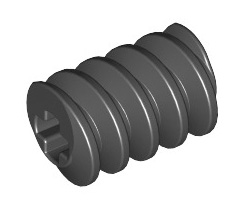
\includegraphics[width=\textwidth]{gears/worm}
\caption{Snekke}
\label{gearing:snekke}
\end{subfigure}
%\begin{subfigure}[b]{.19\textwidth}
%\centering
%
\includegraphics[width=\textwidth]{gears/16-tooth}
%\caption{16-tands}
%\label{gearing:16tand}
%\end{subfigure}
\begin{subfigure}[b]{.19\textwidth}
\centering

\includegraphics[width=\textwidth]{gears/24-tooth}
\caption{24-tands}
\label{gearing:24tand}
\end{subfigure}
\begin{subfigure}[b]{.19\textwidth}
\centering
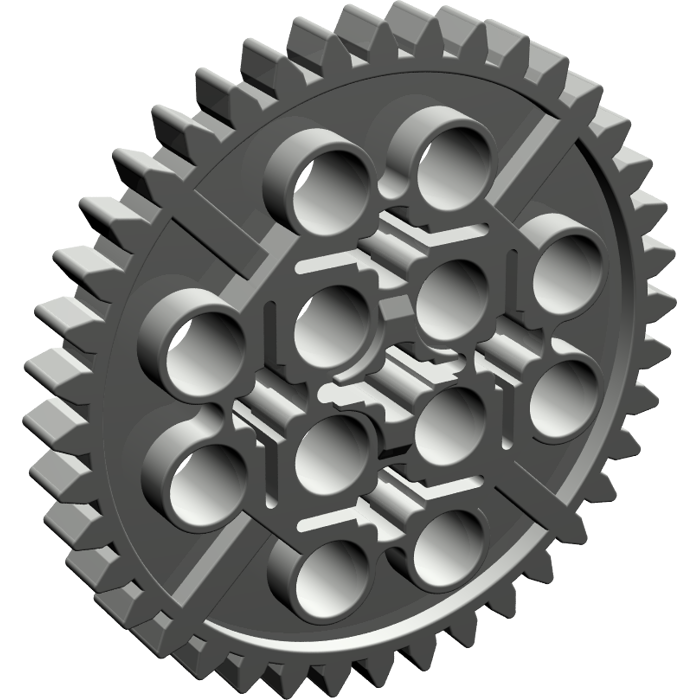
\includegraphics[width=\textwidth]{gears/40-tooth}
\caption{40-tands}
\label{gearing:40tand}
\end{subfigure}
\caption{De anvendte tandhjul til sensor rotation.}
\label{gearing:tandhjul}
\end{figure}

Den første kombination består af en snekke\cite{snekke} (se \cref{gearing:snekke}) som fører-tandhjul og 24-tands (se \cref{gearing:24tand}) som følger-tandhjul.
Snekken kræver en hel rotation for at flytte én tand på følger-tandhjul, hvilet giver en gear ratio på $1:24$, som betyder, at der kræves 24 hele motor-rotationer for at rotere 24-tands (følger) tandhjulet én omgang.

Den anden kombination består af et 24-tands (se \cref{gearing:24tand}) som fører-tandhjul og et 40-tands (se \cref{gearing:40tand}) som følger-tandhjul, hvilket giver en ratio på $1:1.667$.

Den samlede gear ratio for sensor motoren bliver derfor $1:40$, som beskriver, at der for hver sensor omdrejning kræves 40 motor omdrejninger; hvilket er det samme som:
$$\frac{24}{1} \cdot \frac{40}{24} = 40$$